\section{Data assimilation}

\subsection{Introduction}
\noindent Data assimilation is nowadays widely used to make predictions in complex systems, for example in weather forecasting or ocean simulation. Data assimilation is a method that combines observations with the output of a model to improve a prediction. 
The main idea is to combine information from our model and from observations, in order to have a more reliable analysis. Sometimes the output of the model may not be in the same space as the observations. This is something that we need to consider while doing our assimilation. This means that there will be uncertainties coming from the model or from the observations, as were asthese uncertainties coming from our input that will also translate into uncertainties in our output.
At the end of the data assimilation we will obtain an output which will be an estimate of the unknown  state variables.
The best estimate is searched for as a linear combination of the background estimate and the observations:

$$x^a=Lx^b+Ky^0$$


\noindent Data assimilation methods are often split into two families: statistical methods and a variational methods.
For the internship we will be focusing on the statistical methods.
\subsection{Statistical approach}
\subsubsection{Kalman filter}
The Kalman filter method consists in looking for an analyzed state $x^a$ . This analysis will be a linear combination of the outputs of the model and observations.
To explain this method let's consider that we observe a single quantity, an estimation of a scalar quantity at a point in space. For example we are observing the temperature in the middle of the room, and the model also outputs the temperature in the middle of the room.  We will then have :
$$x^a=x^b+K(y-x^b)$$
with $x^a=\begin{pmatrix}
 x_1^a  \\ 
 \vdots \\
 x_n^a \\
\end{pmatrix}$ the analysis, $x^b=\begin{pmatrix}
 x_1^b  \\ 
 \vdots \\
 x_n^b \\
 \end{pmatrix}$ the state background or model output, $y=\begin{pmatrix}
 y_1  \\ 
 \vdots \\
 y_p \\
 \end{pmatrix}$ the observation and $K$ the gain matrix of size $p \times p$. 

\noindent To simplify let's consider that we are trying to find the true state in the scalar setting (1D), we suppose that the true state $x^t$ exists so:
$$x^a-x^t=x^b-x^t+K(y-x^t-x^b+x^t).$$
Let's define the errors:
$$\begin{aligned}
&\epsilon^a=x^a-x^t, \\
&\epsilon^b=x^b-x^t, \\
&\epsilon^y=y-x^t. \\
\end{aligned}$$
So we will have:
$$\epsilon^a=\epsilon^b+K(\epsilon^y-\epsilon^b).$$
If we have many realisations of these error, then we can write:
$$<\epsilon^a>=<\epsilon^b>+K(<\epsilon^y>-<\epsilon^b>).$$
We want to have the analysis error variance as low as possible .So we want to minimize $<(\epsilon^a)^2>$ with respect to $K$, this will give us:
$$<(\epsilon^a)^2>=<(\epsilon^b)^2>+K^2<(\epsilon^y-\epsilon^b)^2>+2K<\epsilon^b(\epsilon^y-\epsilon^b)^2>,$$
$$2K<(\epsilon^y)^2+(\epsilon^b)^2>-2<(\epsilon^b)^2>=0.$$
\noindent We assume that the errors in the background and observation are uncorrelated,wh,ch leads to
$$K=\frac{<(\epsilon^b)^2>}{<(\epsilon^b)^2>+<(\epsilon^y)^2>} \Rightarrow K=\frac{(\sigma^b)^2}{(\sigma^b)^2+(\sigma^y)^2}, $$
where $(\sigma^y)^2$ is the observations error variance and $(\sigma^b)^2$ is the background or model error variance.
\newline\noindent If we have $(\sigma^y)^2=0$, $K=1$ and $x^a=y$  this means that the observation are perfect.
\newline\noindent And if $(\sigma^b)^2=0$, $K=0$ and $x^a=x^b$ this is equivalent to ignoring the observations.
\vspace*{5mm}
\newline Now that we have explained the method for finding $x^a$ in the 1D case, let's try to generalize our formula in a multi-dimensional case:

$$\left\{\begin{aligned}
		&x^a=(I-KH)x^b+Ky^0=x^b+K(y^0-H(x^b)), \\
        &K=BH^T(HBH^T+R)^{-1}. \\
	\end{aligned}\right.$$
With $K$ the gain or weight matrix, $(y^0-H(x^b))$ the innovation and $H$ the linear operation of the observations.
This formulation is called the Best Linear Unbiased Estimator (BLUE) or least squares analysis.
The principle of the Kalman filter is based on this formulation. Here is a small figure which illustrates the Kalman filter.
\vspace*{5mm}
\begin{figure}[H]
    \centering
		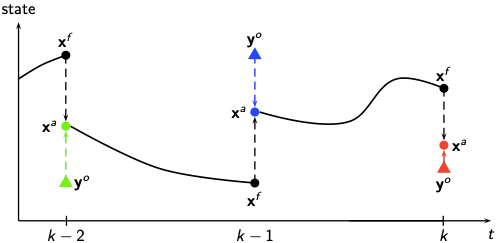
\includegraphics[width=0.8\textwidth]{"images/enkf/schema_kalman_filter.png"}
	\caption{Kalman filter}
\end{figure}
The general idea consists in estimating the state at time $k$ from an estimate at time $k-1$ and measurements at time $k$.
We do the estimation in two steps:
\begin{enumerate}[label=\textbullet]
		\item Prediction of the state from the evolution model
		\item Correction of the prediction from the measurements
	\end{enumerate}

\subsubsection{Kalman filter algorithm}
Let us precise the notations we will use.
\newline
\noindent Let $n\in \mathbf{N}$ be the state's size, $k\in \mathbf{N}$, $x_k^f ,x_k^a\in \mathbf{R^n}$ and $P_k^f,P_k^a \in \mathbf{R^{n\times n}}$:
 \begin{enumerate}[label=\textbullet]
		\item $k\in \mathbf{N} $ the time index
		\item $x_{k}^{f}\in \mathbf{R^n}$ forecast state (background), forecast error covariance matrix $P_{k}^{f}\in \mathbf{R^{n\times n}}$
		\item $x_{k}^{a}\in \mathbf{R^n}$ analyzed state (result of the assimilation process), analysis error covariance matrix $P_{k}^{a}\in \mathbf{R^{n\times n}}$
	\end{enumerate}
\noindent Let us define the operators:
    \begin{enumerate}[label=\textbullet]
		\item model operator $ M_{k,k+1}(x_{k}^{t}) $ model error $\eta
		_{k,k+1}$, covariance matrix $Q_k\in \mathbf{R^{n\times n}}$
		\item observation operator $ H_k (x^t ): \mathbf{R^n} \rightarrow \mathbf{R^n} $ , observation error $\epsilon^0\in \mathbf{R^n}$, covariance matrix $R_k\in \mathbf{R^{n\times n}}$
	\end{enumerate}
\noindent The hypotheses necessary for the application of the Kalman filter are:
    \begin{enumerate}[label=\textbullet]
		\item Model and observations operators $M_{k,k+1}$ and $H_k$ are linear.
		\item Errors are unbiased, Gaussian, independent and white in time. For example for the observation we will have $<\epsilon_k^0\epsilon_j^{0T}>=0$ if $k\ne j$:.
	\end{enumerate}
So finally we obtain the Kalman filter algorithm.
\begin{enumerate}[label=(\roman*)]
\item Initialization: $x_0^f$ and $P_0^f$ are given, equal to $x^b$ and $B$
\item BLUE:
$$\begin{aligned} &K_k=(H_kP_k^f)^T[H_k(H_kP_k^f)^T+R_k]^{-1} \\
&x_k^a=x_k^f+K_k(y_k^0-H_kx_k^f) \\
&P_k^a=(I-K_kH_k)P_k^f \\
\end{aligned}$$

Forecast step:
$$\begin{aligned} 
&x_{k+1}^f=M_{k,k+1}x_k^a \\
&P_{k+1}^f=M_{k,k+1}P_k^aM_{k,k+1}^T+Q_k\\
\end{aligned}$$
\end{enumerate}

\subsection{Ensemble Kalman Filter}
\subsubsection{Explanation of the method}
\noindent We have seen so far two methods to do data assimilation, these methods are valid only for linear systems, but the Lorenz system is non-linear, that's why we will introduce the Ensemble Kalman Filter method which works well for non-linear systems. The ENKF method consists in using the Kalman filter method in high dimension and compare P by a set of states $x_1,x_2,..,x_{m}$. So we can approximate the moments of the error by the moments of the sample.
For all the samples, we have:
$$x_i^a=x_i^f+K[y-h(x_i^f)]$$
with $h(x_i^f)$ the observation operator.
\newline \noindent To begin with we can estimate the
forecast error covariance matrix as:
$$P^f=\frac{1}{m-1}\sum_{i=1}^{m}(x_i^f-\bar{x}^f)(x_i^f-\bar{x}^f)^T~~with~~\bar{x}^f=\frac{1}{m}\sum_{i=1}^{m}x_i^f .$$ 
\noindent We can factorized the forecast error covariance matrix by:
$$P^f=X_f X_f^T$$
where $X_f$ is an $n \times m$ matrix whose columns are the normalized anomalies or normalized perturbations,
$$[X_f]_i=\frac{x_i^f-\bar{x}^f}{\sqrt{m-1}}$$

\noindent We can also define the Kalman gains: 
$$K=P^f H^T(HP^f H^T+R)^{-1}$$

\noindent In addition, we have:
$$
\bar{x}^a=\frac{1}{m}\sum_{i=1}^mx_i^a~~,~~~~[X_a]_i=\frac{x_i^a-\bar{x}^a}{\sqrt{m-1}} $$
\subsection{Presentation of the results}
\subsubsection{Harmonic oscillator}
\noindent After the implementation for the data assimilation, to test it, the idea was to find an equation for which we know the exact result. That's why we chose to test it with the harmonic oscillator equation:
$$\qquad \frac{\partial x}{\partial t}=v \quad \Rightarrow \quad \frac{\partial^2 x}{\partial t^2}=\frac{\partial v}{\partial t}$$

\IncMargin{1em}
\begin{algorithm}
\SetKwData{Left}{left}\SetKwData{This}{this}\SetKwData{Up}{up}
\SetKwFunction{Union}{Union}\SetKwFunction{FindCompress}{FindCompress}
\SetKwInOut{Input}{input}\SetKwInOut{Output}{output}
\Input{For k=0,...,K: the observation error covariance matrices $R_k$, the observation models $H_k$, the forward models $M_k$.}

\BlankLine
Initialize the ensemble$\left\{x_{i,0}^f \right\}_{=1,...,m}$\;
\For{$k$=0,...,K}{
Draw a statistically consistent observation set: \newline for i=1,...,m: $y_{i,k}=y_k+u_i$, with $u_i \sim \mathcal{N}(0,R_k)$\;
Compute the ensemble means
\newline $\bar{x}_k^f=\frac{1}{m}\sum_{i=1}^{m}x_{i,k}^f $, $\bar{u}=\frac{1}{m}\sum_{i=1}^{m}u_{i}$,$\bar{y}_k^f=\frac{1}{m}\sum_{i=1}^{m}H_k(x_{i,k}^f) $
\newline and the normalized anomalies
\newline $[X_f]_{i,k}=\frac{x_{i,k}^f-\bar{x}_{k}^f}{\sqrt{m-1}}$, $[Y_f]_{i,k}=\frac{H_k(x_{i,k}^f)-u_i-\bar{y}_{k}^f+\bar{u}}{\sqrt{m-1}}$\;
Compute the gain: $K_k=X_k^f(Y_k^f)^T \left\{ Y_k^f(Y_k^f)^T\right\}^{-1}$\;
Update of the ensemble:
\newline for i=1,...,m: $x_{i,k}^a=x_{i,k}^f+K_k(y_{i,k}-H_k(x_{i,k}^f))$\;
Compute the ensemble forecast:
\newline for i=1,...,m: $x_{i,k+1}^f=M_{k+1}(x_{i,k}^a)$
}
\caption{Ensemble Kalman Filter}\label{enkf}
\end{algorithm}
\subsection{Comparison of Python results with C++}
\noindent During the project we used a function already implemented in the library Filterpy  to perform data assimilation. In the internship we had to implement it in C++. In order to verify the results we obtained with the C++ implementation, we wrote in csv files our observation, model and analized state for each time step and then read them back in Python. Having both results (C++ and Python) in Python makes the comparison easier.


\noindent For this case, the model and the observation will be the Lorenz system solved with RK4, we chose to take exactly the same initial point but different parameters for the observations and the model. For $(\sigma, r, b)$ we have chosen to take $(12.,6.,12.)$ for the observation and $(10.,6.,10.)$ for the model. For the initial condition we have taken for both $(-10,10,25)$. 
\newline \noindent The Lorenz system: 
$$
	\begin{cases}
		
		x'&=\sigma(y-x) \\
		y'&=x(r-z)-y \\
		z'&=xy-bz
		
	\end{cases}
	$$
 \begin{figure}[H]
        \centering
		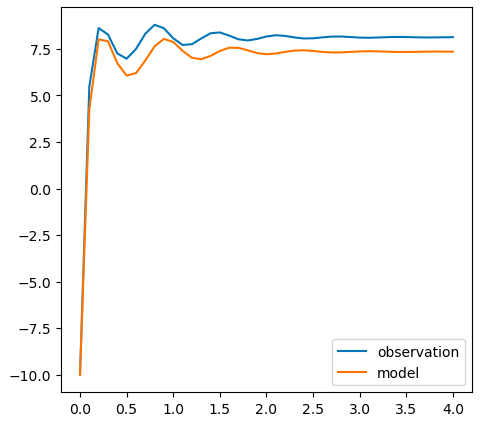
\includegraphics[width=0.5\textwidth]{"images/enkf/result.png"}
		\caption{Lorenz system example, $(\sigma, r, b)=(12.,6.,12.)$, $X_0=(-10.,-10.,25.) $ for observation and $(\sigma, r, b)=(10.,6.,10.)$, $X_0=(-10.,10.,25.)$  for the model}
\end{figure}

\noindent\newline Let's take 
			$$P=\begin{pmatrix}
            0.1 & 0. & 0. \\
            0. & 0.1 & 0. \\
            0. & 0. & 0.1 \\
            \end{pmatrix} ,
            Q=\begin{pmatrix}
            0.1 & 0. & 0. \\
            0. & 0.1 & 0. \\
            0. & 0. & 0.1 \\
            \end{pmatrix},
            R=\begin{pmatrix}
            0.01 & 0. & 0. \\
            0. & 0.01 & 0. \\
            0. & 0. & 0.01 \\
            \end{pmatrix}.$$ 
 \begin{figure}[H]
        \centering
		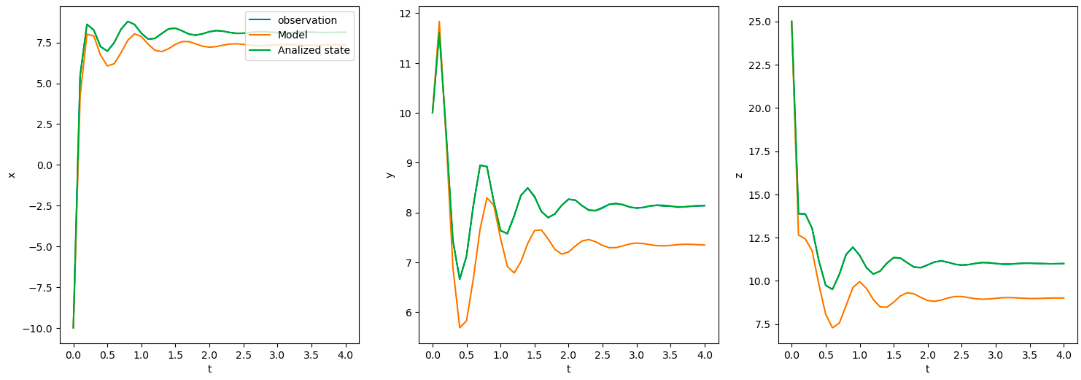
\includegraphics[width=1\textwidth]{"images/enkf/result_filterpy.png"}
		\caption{Curve of the model, observation and analyzed states with Filterpy}
\end{figure}
 \begin{figure}[H]
        \centering
		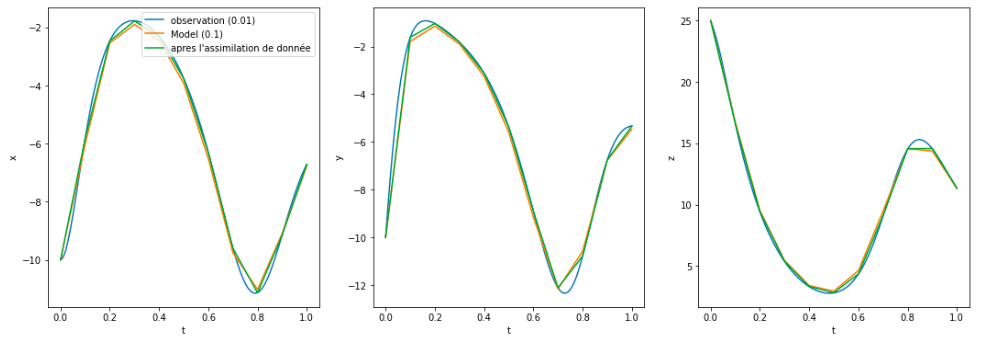
\includegraphics[width=1\textwidth]{"images/enkf/result_cpp.png"}
		\caption{Curve of the model, observation and analyzed states with C++}
\end{figure}
\noindent
First of all let's try to understand the impact of the covariance matrices associated with the error in the algorithm. For this  case we took a covariance matrix associated to the observation R smaller than the other matrices. This refers to the fact that our observations are very precise, and are much closer to the exact solution. For Q, the covariance matrix associated to the model, we have also chosen diagonal matrix, with 0.1 on all the entries, since we solve it with the method of RK4 this one remains quite accurate. And for P,  we have chosen  diagonal matrix, with 0.1 on all the entries.
\newline
\noindent We expect to see that our green curve is close to the blue curve which corresponds to the observations. On the other hand we notice that the values of the states after the data assimilation are very close almost similar to the observation ones.
\newline \noindent We can also notice that our results obtained with Filterpy and with the implementation made with C++ are very similar. This proves us that our implementation in C++ seems to work properly.


\newpage
\subsection{Integrate data assimilation to Feel++ toolboxes}
\subsubsection{The context}
\noindent For the second part of the internship, our goal was to integrate the Ensemble Kalman Filter algorithm to Feel++ toolboxes. For this we had to realize a simulation of an office located in the university of Strasbourg, at the UFR of mathematics on the 2nd floor. This simulation will be the model to be used for data assimilation, and it will return the temperature of the office for a given time and at each point of the room. 
\newline \noindent To perform data assimilation, apart from a numerical model (obtained with Feel++) we also need observations. For the observation we have 10 sensors in the office that collect the temperature every hour. 

 \begin{figure}[H]
        \centering
		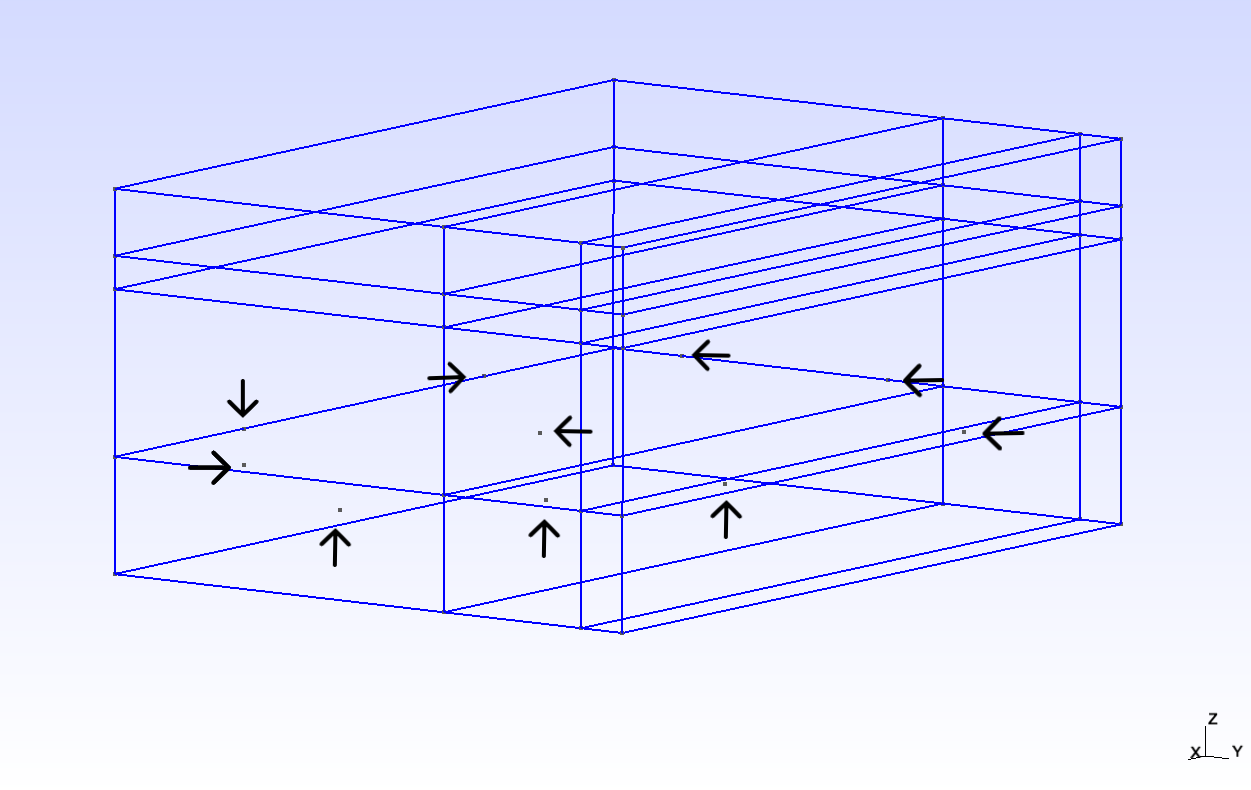
\includegraphics[width=0.7\textwidth]{"images/enkf/Maillage_1.png"}
		\caption{Mesh of the office with the 10 sensors}
\end{figure}
 \begin{figure}[H]
        \centering
		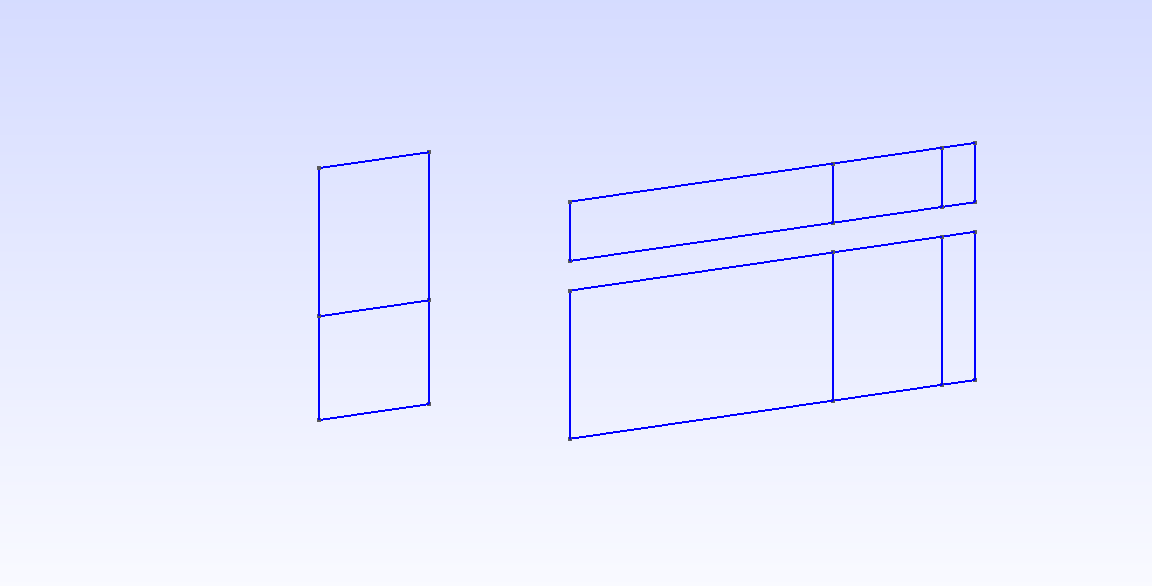
\includegraphics[width=0.6\textwidth]{"images/enkf/Maillage_2.png"}
		\caption{Mesh of the office with the 10 sensors:View of the windows and door}
\end{figure}
\subsubsection{Heat flux}
\noindent In order to simulate the evolution of the temperature in the office, we must first understand the different types of heat transfer. Heat transfer is one of the modes of internal energy exchange between two systems. Heat goes always from a hot body to a cold one and it takes place until the two systems or two bodies are at the same temperature. When the two bodies are at the same temperature, we call this " thermal equilibrium", the two systems are at the same temperature and there is no more heat transfer between the two systems.

 \begin{figure}[H]
        \centering
		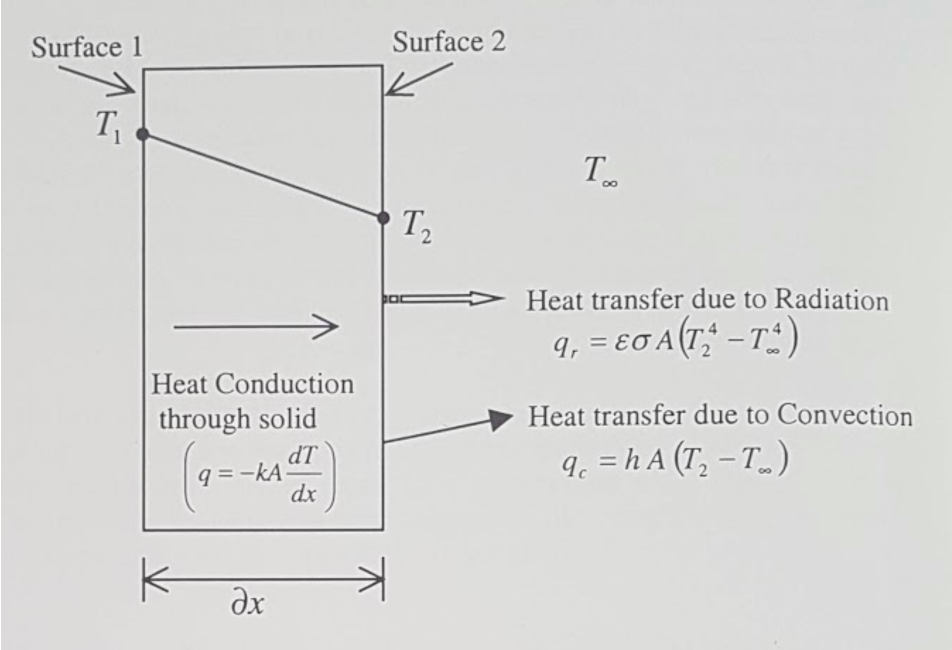
\includegraphics[width=0.8\textwidth]{"images/enkf/flux_1.png"}
		\caption{Three different modes of heat transfer}
\end{figure}
\newline\noindent There are three kinds of heat transfer:  the first is conduction, it is the heat transfer that takes place when two solid bodies are in contact. 
 \begin{figure}[H]
        \centering
		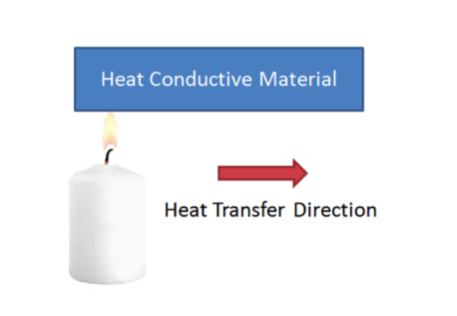
\includegraphics[width=0.6\textwidth]{"images/enkf/flux_2.png"}
		\caption{Conduction}
\end{figure}
\noindent 
This is the simplest type of heat transfer and the law that applies to conduction is Fourier's law, which states that the heat flux is of the form $Q=-k\nabla T$. In a building, this kind of heat transfer takes place inside walls, or between any pair of solid objects at different temperatures.
\newline\noindent The second type of heat transfer is convection. Convection occurs when a fluid participates in the heat transfer.
\begin{figure}[H]
        \centering
		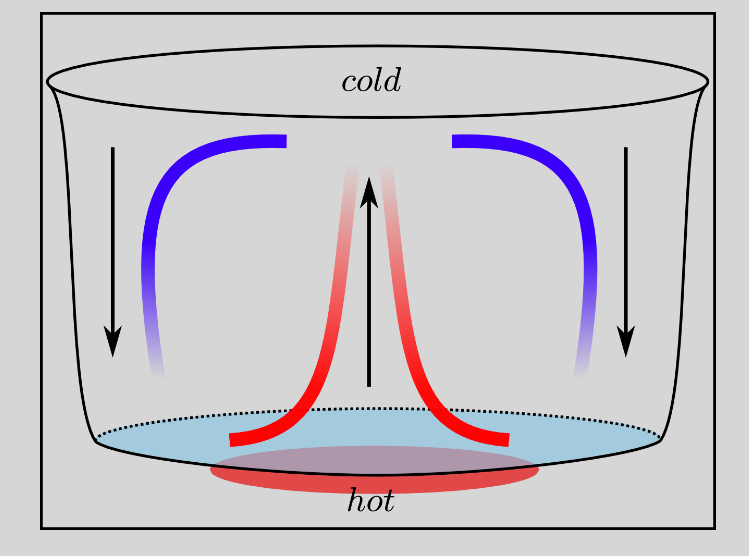
\includegraphics[width=0.5\textwidth]{"images/enkf/flux_5.png"}
		\caption{Convection}
\end{figure}
\noindent In convection, heat is transferred by the motion of matter. In a building, for example, convective heat exchange takes place when hot/cold air masses enter from the window. An another example can be when we heat water, the hot water which has a lower density at the bottom will go up, and conversely the cold water which is at the top will go down and we will see the appearance of convection rolls. 
\newline \noindent The third type of heat transfer is the radiation.
  \begin{figure}[H]
        \centering
		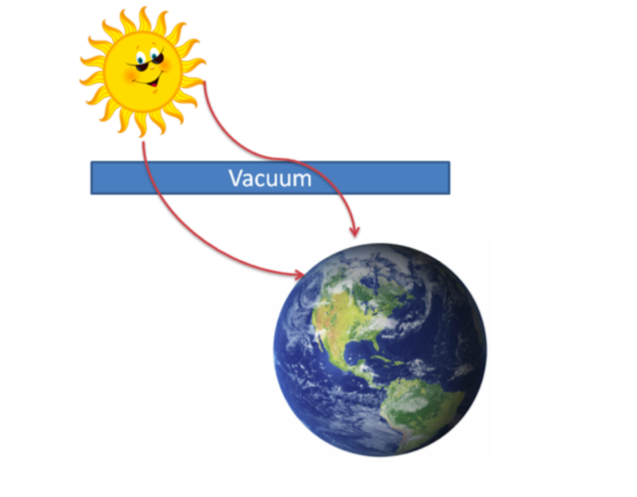
\includegraphics[width=0.6\textwidth]{"images/enkf/flux_4.png"}
		\caption{Radiation}
\end{figure}
\noindent Radiation is the only energy transfer that takes place in vacuum. It is the light which will transport the energy, it will be transported either as an electromagnetic wave or as a photon. In building simulations, the most important source of heat from radiation is the sun, whose beams hit the building opaque walls and enter the interior space through transparent surfaces.
Consequently, any object emits a radiation. 
     \begin{figure}[H]
        \centering
		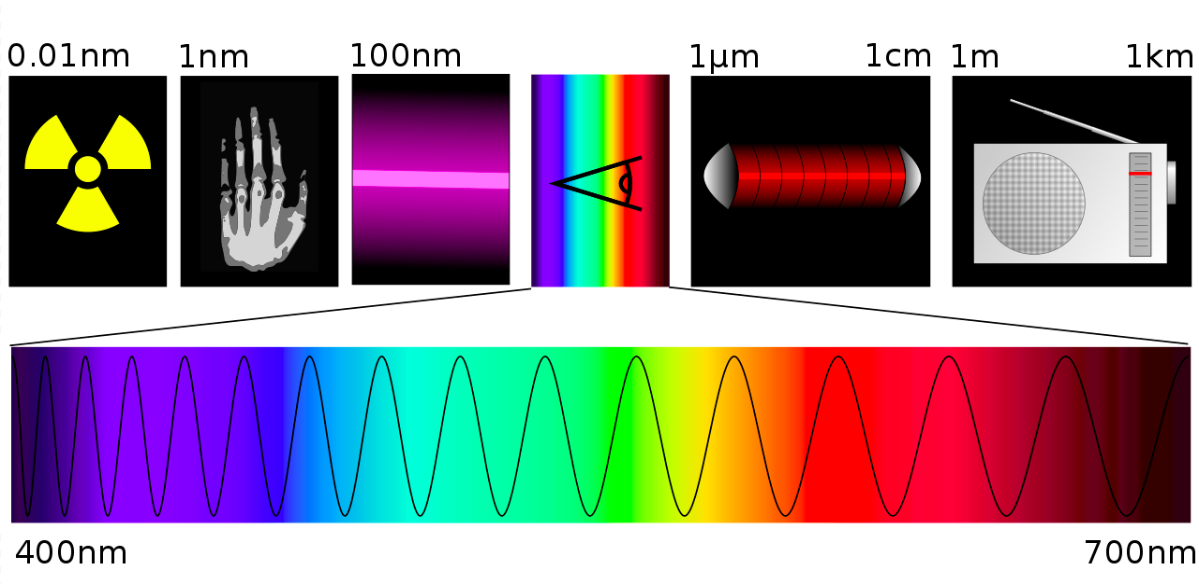
\includegraphics[width=0.6\textwidth]{"images/enkf/flux_3.png"}
		\caption{Electromagnetic spectrum}
\end{figure}
\subsubsection{The simulation using Feel++ toolboxes}
\noindent Feel++ is a powerful tool for numerical simulations. 
Using JSON and CFG files, we can configure models by defining the required parameters like physical quantities, material properties, constants. It is possible to solve several types of problems like stationary or time dependent, linear or non linear. It's also possible with Feel++ to realize solutions with several cores for larger problems.
\newline
\newline
\newline\noindent To study the heat flow in the office we want to simulate, we must first study the heat equation with convective effects.  
\begin{itemize}
    \item Heat equation with convective effects.

 $$\rho C_p((\frac{\partial T}{\partial t})+u \cdot \nabla T)-\nabla \cdot (k \nabla T)=Q$$
\noindent Which is completed with boundary conditions, initial value and with the parameters below.
\newline
\newline
\newline
\renewcommand{\arraystretch}{2}
\begin{tabular}{|R{3cm}|C{5cm}|L{3cm}|L{3cm}|}
\hline
$\rho$ & Air density & $Kg.m^
{-3}$ & 1.125  \\[0.5cm]
\hline
$C_p$ & Specific heat & $J/KgK$ & 1004 \\[0.5cm]
\hline
$k$ & Conductivity & $W/mK$ & 0.025  \\[0.5cm]
\hline
$u$ & Fluid velocity & $m.s^{-1}$ & unknown \\[0.5cm]
\hline
\end{tabular}
\end{itemize}

\noindent The real unknown in our case will be the temperature, but we can see that there is a second unknown in this equation which is the fluid velocity. This unknown comes from the fact that we have chosen to work with the heat equation with convective effects. In order to find this value it will be necessary to use other equations, which are the Navier-Stokes equations.
\newline
\newline \noindent In fluid mechanics, the Navier-Stokes equations are nonlinear partial differential equations that describe the motion of fluids in the continuous state. They apply to the motion of air in the atmosphere, ocean currents, the flow of water in a pipe, and many other fluid flow phenomena. 
\begin{itemize}
\item Equation of the air motion (Navier-Stokes).
 $$\left\{\begin{aligned} 
        &\rho (\frac{\partial u}{\partial t}+u \cdot \nabla u)-\nabla \cdot (\mu \nabla u)+\nabla P =-\rho_0 \beta(T-T_{ref})g\\
        &\nabla \cdot u=0 \\
    \end{aligned}\right.$$
\renewcommand{\arraystretch}{2}
\begin{tabular}{|R{3cm}|C{5cm}|L{3cm}|L{3cm}|}
\hline
$\rho$ & fluid density & $Kg.m^
{-3}$ & 1.125 \\[0.7cm]
\hline
$u$ & fluid velocity & $m.s^{-1}$ & unknown \\[0.7cm]
\hline
$\beta$ & coefficient of thermal expansion & $K^
{-1}$ &  0.0034 \\[0.7cm]
\hline
$\mu$ & dynamic viscosity & $Pa.s$ & $1.81e^{-5}$\\[0.7cm]
\hline
$g$ & gravitational acceleration & $m.s^{-2}$ & $9.8$\\[0.7cm]
\hline
\end{tabular}
\end{itemize}
\noindent 
In order to simulate our office we have to solve two different equations, first we have to solve the Navier-Stokes equations in order to find the dynamic viscosity and reinject this value in the heat equation to finally find the temperature. 
\newline \noindent To achieve this we can first use the Heat Transfer and Fluids toolboxes to find the dynamic viscosity $\mu$, then use the Heat Transfer toolbox by injecting the value found by applying the Fluid toolbox to find the temperature in the room for each time step.
\newline\noindent However, for the rest of the internship, in order to facilitate the problem and to save time, we have chosen to solve the heat equation without convection effect.
\begin{itemize}
    \item Heat equation without convection effect.

 $$\rho C_p(\frac{\partial T}{\partial t})-\nabla .(k \nabla T)=Q$$
\noindent Which is completed with boundary conditions, initial value and the values of the chosen parameters are typical for air.
\end{itemize}
\noindent We chose to take a time step of 10 minutes for the simulation and we put radiation coming from the windows. For the outside temperature we put it at 27,85 degrees celsius, and we initialize the temperature inside the room to 20 celsius.
\begin{figure}[H]
        \centering
		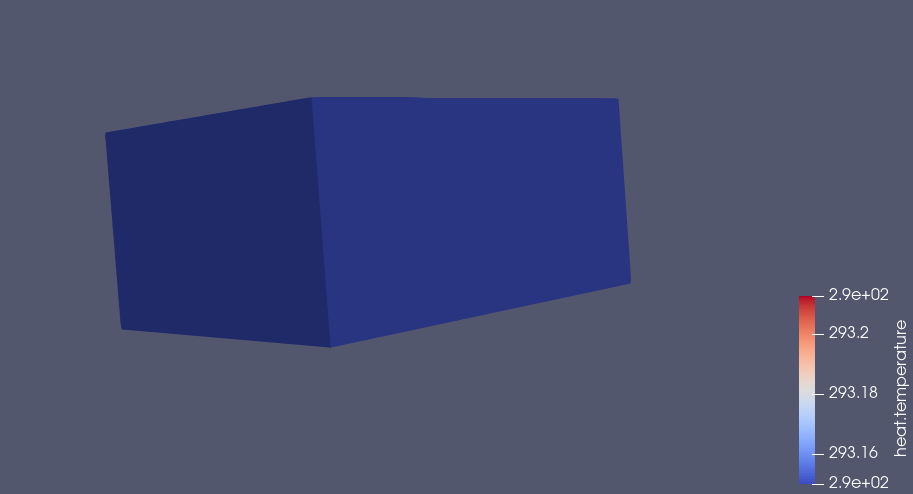
\includegraphics[width=0.6\textwidth]{"images/enkf/sim_1.png"}
		\caption{Simulation realized with the toolbox heat of Feel++ (time= 0)}
\end{figure}
\begin{figure}[H]       
	\begin{minipage}[t]{0.47\linewidth}
		\centering
		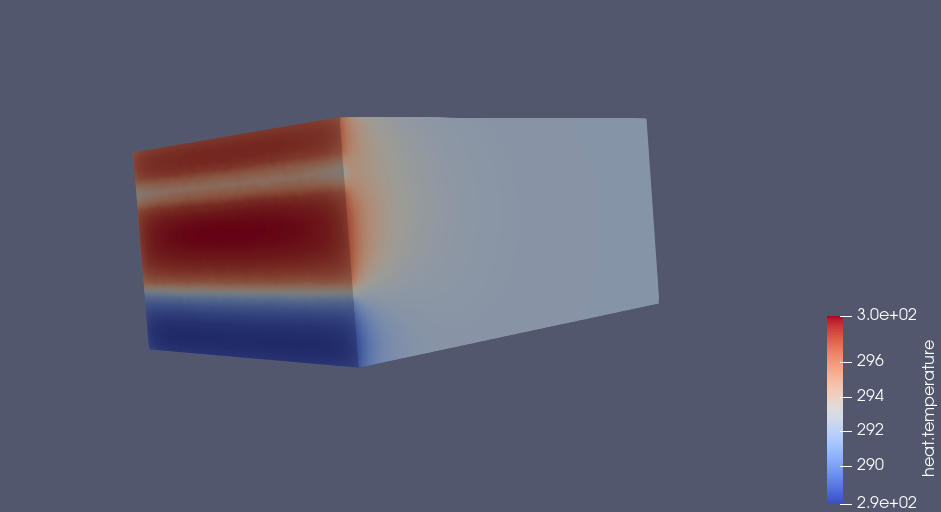
\includegraphics[width=\linewidth]{"images/enkf/sim_3.png"}
	\end{minipage}
	\begin{minipage}[t]{0.48\linewidth}
		\centering
		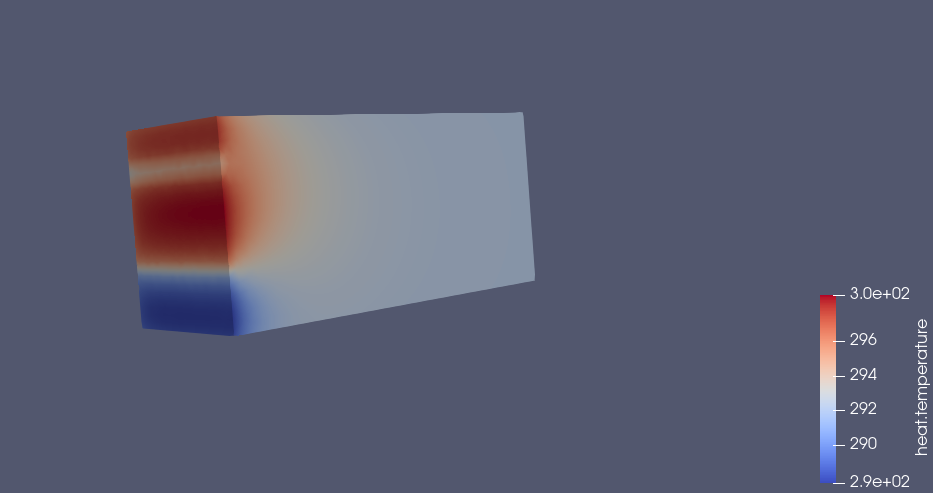
\includegraphics[width=\linewidth]{"images/enkf/sim_4.png"}
	\end{minipage}
	\captionof{figure}{Simulation realized with the toolbox heat of Feel++ (time= 1h.)}
	\label{lorenz:exact3D}
\end{figure}
\noindent We notice that at the beginning of the simulation the office is at 20 degrees everywhere, which means that the simulation has taken into account the initial condition that we had given. We notice that after one hour, we have radiation coming from the windows. We can see the heat source beginning to warm up the room. This is due to the fact that during the simulation we had set the radiation factor for the windows. We can also see that the heating of the room is done very slowly. The reason for this is that we have ignored the convective effects.
\newpage
\subsubsection{Including data assimilation to our simulation}
\noindent In the previous sections we have seen how to build our model using the toolboxes available in Feel++. We have also seen how to get the observations from the 10 sensors located in the office. Now let's try to understand how to apply our Ensemble Kalman Filter class to correct our simulation with our sensor data. To do this let's first try to understand how to use our ENKF class. 
\newline\noindent The Ensemble Kalman Filter  class is composed of 3 major functions. 
\newline\noindent The first one is the initialization. This one takes in arguments all the necessary parameters in order to initialize them. It takes: 
\begin{itemize}
    \item the dimension of our model, in our case it will be of size 10 because we have 10 sensors in our office;
    \item the dimension of the vector containing our observations which will also be of size 10 for the same reason;
    \item we will have a vector X of size 10 which will represent the initial state for our model;
    \item the matrix P which will be the covariance matrix associated to the analyzed state;
    \item our time step dt. For our case we have chosen to perform the data assimilation every hour because the observations are available for each hour;
    \item a function \text{hx} which takes a state as argument, and it allows us to pass from the model space to the observation space. For our example they are the same dimension;
    \item and finally a function \text{fx}, which takes as arguments the time, the state, the index of the sample to be simulated and the time step. It returns the state for the next time step;

\end{itemize}
\noindent The second function in our class is the predict function. To summarize, this function will predict the state of each sample for the next time step. This is where our \text{fx} function is used. 
The last function, named update takes as argument an observation vector z, and calculates the analyzed state. 
\newline
\newline \noindent The delicate part to realize the data assimilation was to create the \text{fx} function. In the case of Lorenz it was obvious, this function was only applying RK4 to find the state for the next time step. For our case, we have to apply the simulation using as initial point our state in argument. But to implement this function, we had to pay attention to several points. 
\begin{itemize}
    \item First of all, in order to perform simulations using toolboxes in Feel++, we need to give it as initial condition a h5 file where the temperature of the office at each mesh point is stored. When we run simulations in Feel++, the toolboxes automatically generate h5 files for each time step. These files are only readable by Feel++. But the tricky part is that our vector X given as argument in the function \text{fx} stores only the temperature at the points where the sensors are located. But in order to realize the simulation we need instead a vector field where are stored the temperature at each point of the office. We have to modify our h5 file in order to integrate the temperature values at the sensors positions (which are in the X vector). The approach we choose is to apply Gaussian  $\frac{1}{\sigma \sqrt{2 \pi}}\exp ^{-\sum \frac{\|x-\mu\|}{2 \sigma^2}}$ around our sensors for a given radius to make a more general and accurate correction.
   
    \item After modifying our h5 file with the Gaussians around the sensors, we need to perform the simulation to get our state for the next time step. Therefore thanks to the toolboxes in Feel++, by giving as initial condition our modified h5 file we will be able to get our state for the next time step. This will also be stored as a h5 file, and to pass from the temperature field to point values, we chose to average the finite element field around the sensors.  
    \item The last important point was the fact that we applied the \text{fx} function to each sample. As explained before, our Ensemble Kalman Filter applies the Kalman Filter to each sample. But in our case, we have to give him a h5 in order to apply the simulation. The solution we found for this problem is to put in argument to the \text{fx} function the sample index. To avoid the files to be overwrite at each simulation, we have created directories for each sample to store the h5 files. And when we will apply our \text{fx} function, this one will be able to get the h5 file corresponding to the right sample.
\end{itemize}
\noindent Taking into account all these points, we have implemented the function \text{fx}. However after several debugging attempts we did not manage to get it to execute correctly. This function seems to work without returning any error message, but we noticed that we had incorrect values at different places in our vector. Due to the time , we couldn't figure out where the problem was coming from. We think that maybe our Gaussian calculations are falsifying the results, but to be sure, it will be necessary to look in detail at the \text{fx} function.





